% !TeX root = main.tex
\documentclass[a4paper]{article}

\usepackage[
	submission,
	biblatex
]{ducha}
% Switch to [draft,natbib] when you want visible todo notes and BibTeX citations.

\hypersetup{
	pdftitle={User Guide for ducha.sty},
	pdfauthor={Template Maintainer},
	pdfkeywords={LaTeX package, template guide, article workflow}
}

% Author info
\title{\textbf{User Guide for \texttt{ducha.sty}}}
\author{Template Maintainer \\ \email{template@example.com}}
\date{\today}

\duchasetup{
	version=conference,
	license={CC BY 4.0},
	license url={https://creativecommons.org/licenses/by/4.0/},
	copyright={Copyright 2026 Template Maintainer},
	code={Example repository},
	code url={https://github.com/example/ducha-template},
	data={Example dataset},
	data url={https://example.com/data},
	project={Project homepage},
	project url={https://example.com/project},
	preprint={Example arXiv page},
	preprint url={https://arxiv.org/abs/1234.56789},
	doi={10.0000/placeholder-doi},
	note={Replace these placeholder values with the metadata relevant to your release.}
}

\begin{document}
\maketitle

\begin{abstract}
	This document explains how to use the custom package \texttt{ducha.sty}. It shows how to load the package, choose build options, configure version and release metadata, call the helper commands, use the bundled theorem environments, and work with the included table, figure, algorithm, and bibliography support.

	\noindent\textbf{Keywords:} custom package, usage guide, LaTeX template
\end{abstract}

\printduchametadata
\templatelistoftodos

\tableofcontents
% \linenumbers

\section{Quick Start}
\label{sec:quickstart}

Load \texttt{ducha.sty} immediately after the document class. The custom package already configures the page layout, theorem environments, cross-references, figures, tables, algorithms, todo notes, and bibliography support, so a minimal starting point looks like this:

\begin{verbatim}
\documentclass[a4paper]{article}
\usepackage[submission,biblatex]{ducha}
\duchasetup{
  version=journal,
  license={CC BY 4.0},
  code={Repository},
  code url={https://example.com/code}
}

\title{My Document}
\author{Author Name}
\date{\today}

\begin{document}
\maketitle
\printduchametadata
\templatelistoftodos
\tableofcontents
...
\printtemplatebibliography
\end{document}
\end{verbatim}

\cref{sec:options} explains the package options, \cref{sec:metadata} covers version profiles and release metadata, \cref{sec:helpers} shows the helper commands, \cref{sec:theorems} illustrates the theorem and reference setup, and \cref{sec:assets} shows the figure, table, and algorithm support. For broader LaTeX references, see~\cite{lamport1994latex,mittelbach2004latexcompanion}.

\section{Package Options}
\label{sec:options}

The package is controlled by two independent package-option groups: one for review visibility and one for bibliography mode. Rich document metadata such as version, license, copyright, code, and data availability is configured separately with \verb|\duchasetup{...}|.

\begin{table}[ht]
	\centering
	\begin{tabular}{@{}lll@{}}
		\toprule
		\textbf{Option} & \textbf{Effect} & \textbf{Typical use} \\
		\midrule
		\texttt{submission} & Hides todo notes and the todo list & Final or shareable PDF \\
		\texttt{draft} & Shows todo notes and enables the todo list & Internal review build \\
		\texttt{biblatex} & Uses Biber through the package helper & Default workflow \\
		\texttt{natbib} & Uses BibTeX through the package helper & BibTeX-only submission flow \\
		\bottomrule
	\end{tabular}
	\caption{Core options provided by \texttt{ducha.sty}}
	\label{tbl:options}
\end{table}

\begin{table}[ht]
	\centering
	\begin{tabular}{@{}llcc@{}}
		\toprule
		\multirow{2}{*}{Use case} & \multirow{2}{*}{Goal} & \multicolumn{2}{c}{Recommended option} \\
		\cmidrule(lr){3-4}
		 & & Visibility & Bibliography \\
		\midrule
		\multirow{2}{*}{Working draft} & Keep review notes visible & \texttt{draft} & \texttt{biblatex} \\
		 & Match a BibTeX-only workflow & \texttt{draft} & \texttt{natbib} \\
		\multirow{2}{*}{Final output} & Hide review notes & \texttt{submission} & \texttt{biblatex} \\
		 & Hide notes and use BibTeX & \texttt{submission} & \texttt{natbib} \\
		\bottomrule
	\end{tabular}
	\caption{Example option combinations}
	\label{tbl:option-combos}
\end{table}

In practice, most users will start with \verb|\usepackage[submission,biblatex]{ducha}|, switch to \verb|draft| only when they want to surface inline review annotations, and then describe the release itself through \verb|\duchasetup{...}|.

\section{Metadata and Release Profiles}
\label{sec:metadata}

Use \verb|\duchasetup{...}| to declare release metadata without rewriting the package. This is where you specify whether the file is a full version, draft version, conference submission, journal submission, arXiv version, working paper, or some other release profile, along with license, copyright, code, and data information.

\begin{verbatim}
\duchasetup{
  version=conference,
  license={CC BY 4.0},
  license url={https://creativecommons.org/licenses/by/4.0/},
  copyright={Copyright 2026 Author Name},
  code={Project repository},
  code url={https://github.com/user/project},
  data={Companion dataset},
  data url={https://example.com/data},
  project={Project page},
  project url={https://example.com/project},
  preprint={arXiv page},
  preprint url={https://arxiv.org/abs/1234.56789},
  doi={10.0000/example},
  note={Optional internal or public release note.}
}
\end{verbatim}

The current guide file is configured as \textbf{\duchaversionlabel}, which is why the metadata block near the front matter shows a conference-oriented release profile.

\begin{table}[ht]
	\centering
	\begin{tabular}{@{}ll@{}}
		\toprule
		\textbf{Version value} & \textbf{Default printed label} \\
		\midrule
		\texttt{full} & Full Version \\
		\texttt{draft} & Draft Version \\
		\texttt{conference} & Conference Submission \\
		\texttt{journal} & Journal Submission \\
		\texttt{arxiv} & arXiv Version \\
		\texttt{preprint} & Preprint \\
		\texttt{working-paper} & Working Paper \\
		\texttt{tech-report} & Technical Report \\
		\texttt{manuscript} & Manuscript \\
		\bottomrule
	\end{tabular}
	\caption{Built-in release profiles supported by \texttt{\string\duchasetup}}
	\label{tbl:version-values}
\end{table}

\begin{table}[ht]
	\centering
	\begin{tabular}{@{}ll@{}}
		\toprule
		\textbf{Key} & \textbf{Purpose} \\
		\midrule
		\texttt{version} / \texttt{version label} & Select or override the release label \\
		\texttt{license} / \texttt{license url} & Describe the reuse license \\
		\texttt{copyright} & Record ownership or rights text \\
		\texttt{code} / \texttt{code url} & Link the software or repository \\
		\texttt{data} / \texttt{data url} & Link the dataset or archive \\
		\texttt{project} / \texttt{project url} & Link a homepage or landing page \\
		\texttt{preprint} / \texttt{preprint url} & Link a public preprint page \\
		\texttt{doi} & Print a clickable DOI \\
		\texttt{note} & Add a short release-specific note \\
		\bottomrule
	\end{tabular}
	\caption{Metadata keys exposed by \texttt{\string\duchasetup}}
	\label{tbl:metadata-keys}
\end{table}

\section{Helper Commands}
\label{sec:helpers}

\subsection{Document-Level Helpers}
\label{sec:document-helpers}

The package exposes several helpers that matter in most documents:

\begin{verbatim}
\duchasetup{...}
\duchaversionlabel
\email{person@example.com}
\printduchametadata
\templatelistoftodos
\printtemplatebibliography
\end{verbatim}

\begin{itemize}
\item \verb|\duchasetup{...}| stores release metadata such as version, license, code, and data links.
\item \verb|\duchaversionlabel| expands to the current human-readable release label.
\item \verb|\email{...}| creates a clickable mailto link and is useful in the author block.
\item \verb|\printduchametadata| prints the metadata block for the fields you configured.
\item \verb|\templatelistoftodos| prints the todo list only in \texttt{draft} mode.
\item \verb|\printtemplatebibliography| chooses the bibliography command automatically.
It works with both \texttt{biblatex} and \texttt{natbib}.
\end{itemize}

\subsection{Todo Commands}
\label{sec:todo-helpers}

Todo helpers are available in every document, but they only render visibly when the package is loaded with the \texttt{draft} option:

\begin{verbatim}
\Task{Rewrite the introduction}
\TaskPerson{Editor}{Check the notation section}
\TaskDone{Bibliography verified}
\TaskNewPerson{Editor}{Editor}{blue}
\Editor{Rewrite the abstract}
\TaskEditor[highpriority]{Update Figure 2}
\end{verbatim}

This design lets one source file serve both as a collaborative draft and as a clean submission build. In \texttt{submission} mode, these commands are effectively silent.

\subsection{Domain-Specific Math Helpers}
\label{sec:math-helpers}

The package also bundles a set of graph-reconfiguration macros from the original project. If your article is in that area, they are ready to use:

\[
\TS{k}{G},\quad
\TJ{k}{G},\quad
\ReconfSeq{I_0,\dots,I_t},\quad
I \onestep{\sfTS} J,\quad
\dist(u,v),\quad
\CP{n}.
\]

If your document is unrelated to this notation, you can ignore those commands without affecting the rest of the package.

\section{Theorems and Cross-References}
\label{sec:theorems}

The package predefines common theorem-style environments such as \texttt{theorem}, \texttt{lemma}, \texttt{corollary}, \texttt{proposition}, \texttt{definition}, \texttt{example}, \texttt{remark}, and \texttt{problem}. It also loads \texttt{cleveref}, so references are printed automatically with the correct labels.

\begin{definition}
\label{def:configured-doc}
A \emph{configured document} is a \LaTeX{} file that loads \texttt{ducha.sty} and uses its helper commands instead of duplicating preamble setup locally.
\end{definition}

\begin{theorem}
\label{thm:submission-hides-notes}
If a configured document is compiled with the \texttt{submission} option, then review annotations created by the todo helpers do not appear in the output.
\end{theorem}

\begin{proof}
The package wraps the todo commands and the todo list helper in conditional checks on the \texttt{submission} flag. When that flag is true, the visible note-producing branches are skipped.
\end{proof}

\begin{example}
\label{ex:cref}
The sentence ``\cref{def:configured-doc,thm:submission-hides-notes} describe the document setup and its clean-output behavior'' is generated with ordinary \verb|\cref| commands; the package handles the labels automatically.
\end{example}

\begin{remark}
If you need a new theorem-like environment that is not already bundled, add it in the package file so every document using the package receives the same numbering and reference behavior.
\end{remark}

\section{Figures, Tables, and Algorithms}
\label{sec:assets}

The package already loads \texttt{graphicx}, \texttt{booktabs}, \texttt{multirow}, \texttt{tikz}, \texttt{adjustbox}, and \texttt{algorithm2e}. Keep figure assets in \texttt{figs/}; the package sets \verb|\graphicspath{{figs/}}| for you.

\subsection{External Images}
\label{sec:includegraphics}

Typical image commands are available immediately:

\begin{verbatim}

\includegraphics[width=0.45\textwidth]{example}

\includegraphics[height=3cm,keepaspectratio]{example}

\includegraphics[width=0.45\textwidth,trim=1cm 1cm 1cm 1cm,clip]{example}
\end{verbatim}

\begin{figure}[ht]
	\centering
	\begin{minipage}[t]{0.47\textwidth}
		\centering
		\textbf{Width-based scaling}\\[0.5ex]
		
\includegraphics[width=\linewidth]{example}
	\end{minipage}\hfill
	\begin{minipage}[t]{0.47\textwidth}
		\centering
		\textbf{Trimmed and clipped}\\[0.5ex]
		
\includegraphics[width=\linewidth,trim=1cm 1cm 1cm 1cm,clip]{example}
	\end{minipage}
	\caption{Two common \texttt{\string\includegraphics} patterns using \texttt{figs/example.pdf}}
	\label{fig:includegraphics-examples}
\end{figure}

\subsection{TikZ and Width Control}
\label{sec:tikz}

The template wraps TikZ figures in \texttt{adjustbox} so they scale down automatically when they exceed the text width.

\begin{figure}[ht]
	\centering
	\begin{adjustbox}{max width=\textwidth}
		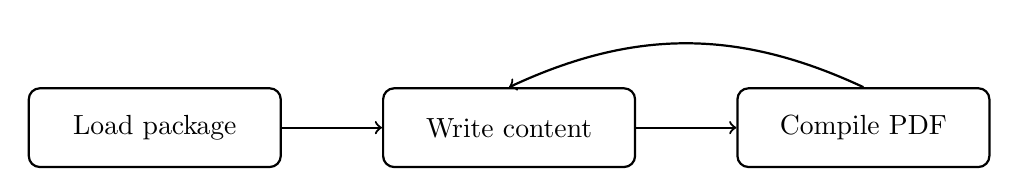
\begin{tikzpicture}[thick]
			\node[draw, rounded corners, minimum width=3.2cm, minimum height=1cm] (load) at (0,0) {Load package};
			\node[draw, rounded corners, minimum width=3.2cm, minimum height=1cm] (write) at (4.5,0) {Write content};
			\node[draw, rounded corners, minimum width=3.2cm, minimum height=1cm] (compile) at (9,0) {Compile PDF};
			\draw[->] (load) -- (write);
			\draw[->] (write) -- (compile);
			\draw[->, bend right=25] (compile.north) to (write.north);
		\end{tikzpicture}
	\end{adjustbox}
	\caption{A simple package-usage workflow drawn directly in the source}
	\label{fig:workflow}
\end{figure}

\subsection{Algorithm Example}
\label{sec:algorithm}

The algorithm environment is ready for methods, procedures, or reproducibility notes:

\begin{algorithm}[ht]
	\caption{Choosing a build configuration}
	\label{alg:workflow}
	\KwIn{A document state, a release target, and a bibliography preference}
	\KwOut{A package option pair plus metadata settings}
	Choose \texttt{draft} if review notes should remain visible; otherwise choose \texttt{submission}\;
	Choose \texttt{biblatex} for the default Biber workflow; otherwise choose \texttt{natbib}\;
	Set \verb|\duchasetup| keys for version, license, copyright, code, and data as needed\;
	Load \texttt{ducha} with the resulting option pair\;
	Print the metadata block if you want that information visible in the front matter\;
	Compile the document and place the bibliography with \verb|\printtemplatebibliography|\;
\end{algorithm}

\section{Bibliography Workflow}
\label{sec:bibliography}

Store bibliography data in \texttt{refs.bib}. The package defaults to \texttt{biblatex} with Biber, but the same source file can switch to \texttt{natbib} with BibTeX by changing the package option:

\begin{verbatim}
\usepackage[submission,biblatex]{ducha}
\usepackage[submission,natbib]{ducha}
\end{verbatim}

Use ordinary citation commands in the body, for example
\cite{lamport1994latex,mittelbach2004latexcompanion}.
Finish the document with \verb|\printtemplatebibliography| so the package can
select the correct bibliography command automatically.

\section{Usage Checklist}
\label{sec:checklist}

When you start a new document with this package, the practical checklist is short:
\begin{enumerate}
\item Load \texttt{ducha} with the right visibility and bibliography options.
\item Use \verb|\duchasetup{...}| to describe the release profile, license, copyright, code, and data information.
\item Keep figure assets in \texttt{figs/} and bibliography data in \texttt{refs.bib}.
\item Place \verb|\printduchametadata| near the front matter if that metadata should appear in the PDF.
\item Place \verb|\templatelistoftodos| near the front matter if you use \texttt{draft} mode.
\item Use the bundled theorem, figure, table, and algorithm environments instead of rebuilding the preamble.
\item End the document with \verb|\printtemplatebibliography|.
\end{enumerate}

\printtemplatebibliography

\end{document}
